\chapter{Sequences and Series of Functions}
\allowdisplaybreaks
\begin{example}
	\label{eg:7.1}
	Bad behaviour of limits
	\begin{enumerate}[label=(\arabic*)]
		\item For $m,n \in \N$, let $p_{m,n}=\frac{m}{n}$.
		      Then
		      \[
			      \lim_{m\to \infty}{p_{m,n}}=\infty
		      \]
		      and
		      \[
			      \lim_{n\to \infty}{p_{m,n}}=0
			      .\]
		      Hence,
		      \[
			      \lim_{n\to \infty}{\underbrace{\lim_{m\to \infty}{p_{m,n}}}_{=\infty}}=\infty \neq \lim_{m\to \infty}{\underbrace{\lim_{n\to \infty}{p_{m,n}}}_{=0}}
			      .\]
		      This shows the order of limits matters.
		\item Let
		      \[
			      f_n(x)=
			      \begin{cases}
				      1    & x\ge 0            \\
				      1+nx & -\frac{1}{n}<x<0  \\
				      0    & x\le -\frac{1}{n}
			      \end{cases}
			      .\]
		      Then $f_n(x)$ is a continuous function.
		      Then $\lim_{n\to \infty}{f_n(x)}= \begin{cases}
				      1 & x\ge 0 \\
				      0 & x<0
			      \end{cases}$, which is not continuous at $0$.
		      This shows that the limit of continuous functions need not be continuous.
		      Moreover,
		      \[
			      \lim_{n\to \infty}{\underbrace{\lim_{x\to 0}{f_{n}(x)}}_{=1}}=1
			      ,\]
		      while
		      \[
			      \lim_{x\to 0}{\underbrace{\lim_{n\to \infty}{f_{n}(x)}}_{=f(x)}}
		      \]
		      does not exist. This shows again that the order of limits matters.
		\item
		      For $x \in [0,1]$, let \[
			      f_n(x)= \begin{cases}
				      1 & n!\cdot x \in \Z    \\
				      0 & n!\cdot x \notin \Z \\
			      \end{cases}
			      .\]
		      Each $f_n \in \mathscr{R}[0,1]$ by Theorem~\ref{thm:6.10}.
		      However, \[
			      f(x)=\lim_{n\to \infty}{f_n(x)}= \begin{cases}
				      1 & x \in Q \cap [0,1]    \\
				      0 & x \notin Q \cap [0,1]
			      \end{cases}
			      .\]
		      Hence, $f(x)$ is nowhere continuous, and $f \notin \mathscr{R}[0,1]$.
		\item
		      Let \[
			      f_n(x)= \begin{cases}
				      0       & \left|x\right|\ge \frac{1}{n} \\
				      n^2x +n & -\frac{1}{n}<x<0              \\
				      -n^2x+n & 0<x<\frac{1}{n}               \\
				      0       & x=0
			      \end{cases}
			      .\]
		      Ten $f(x)=\lim_{n\to \infty}{f_n(x)}=0$ for all $x \in \R$.
		      Moreover,
		      \[
			      \forall{n}: \int_{-1}^{1}{f_n(x)\mathrm{d}x}=1
			      ,\]
		      \[
			      \int_{-1}^{1}{f(x)\mathrm{d}x}=0
			      .\]
		      Hence, $\lim_{n\to \infty}{\int_{-1}^{1}{f_n(x)\mathrm{d}x}}=1\neq  \int_{-1}^{1}{\left(\lim_{n\to \infty}{f_n(x)}\right) \mathrm{d}x}$
		\item Let \[
			      f_n(x)=\frac{\sin{nx}}{\sqrt{n}} \text{ for }  n \in \N, x \in \R
			      .\]
		      Let
		      \[
			      f(x)=\lim_{n\to \infty}{f_n(x)}=0
			      ,\]
		      so
		      \[
			      \forall{x \in \R}: f'(x)=0
			      .\]
		      However, \[
			      f'_n(x)= \frac{n \cos{x}}{\sqrt{n}}=\sqrt{n} \cos{nx}
			      .\]
		      Therefore, $f_{n}'(\pi)=\sqrt{n}(-1)^{n}$ diverges as $n\to \infty$. Hence,
		      \[
			      \underbrace{f'(\pi)=\left(\lim_{n\to \infty}{f_n}\right)^{'}(\pi)}_{=0}\neq \underbrace{\lim_{n\to \infty}{f_n'(\pi)}}_{\text{DNE}}
			      .\]
	\end{enumerate}
	These examples show bad behaviour under interchange of limits, which suggests the need of a stronger notion of convergence.
\end{example}

\begin{define}[7]
	Let $E$ be any set and $f_n: E\to \R (\text{ or } \C) $ for $n \in \N$. Then $f_{n}$ converges uniformly to $f$ on $E$ if \[
		\forall{\epsilon>0}: \exists{N} \text{ s.t. } \forall{n\ge N}: \forall{x \in E}: \left|f_{n}(x)-f(x)\right|<\epsilon
		.\]
\end{define}

\begin{example}
	\begin{enumerate}
		\item
		      Consider the example~\ref{eg:7.1}(2)
		      \[
			      f_n(x)=
			      \begin{cases}
				      1    & x\ge 0            \\
				      1+nx & -\frac{1}{n}<x<0  \\
				      0    & x\le -\frac{1}{n}
			      \end{cases}
			      ,\]
		      \[
			      f_n(x)-f(x)=	\begin{cases}
				      1+nx & -\frac{1}{n}<x<0 \\
				      0    & \text{otherwise}
			      \end{cases}
			      .\]
		      In particular, $f_n(-\frac{1}{2n})-f(-\frac{1}{2n})=\frac{1}{2}$, so we cannot choose $N$ s.t. $n\ge N\implies \left|f_n(x)-f(x)\right|<\epsilon=\frac{1}{4}$ for all $x$.
		      \[
			      \therefore f_n \text{ does not converge uniformly to } f \text{ on } \R
			      .\]
		\item
		      Consider the example~\ref{eg:7.1}(5).
		      \[
			      f(x)=\lim_{n\to \infty}{f_n(x)}=0
			      ,\]
		      \[
			      \forall{x \in \R}: f'(x)=0
			      .\]
		      Then \[
			      \left|f_n(x)-\underbrace{f(x)}_{=0}\right|=\left|\frac{\sin{nx}}{\sqrt{n}}\right|\le \frac{1}{\sqrt{n}}
			      ,\]
		      so $f_n\to f$ uniformly on $\R$.
			      [Note: uniform convergence is not enough for $\lim_{n\to \infty}{f_n'}=(\lim_{n\to \infty}{f_n})'$.]
	\end{enumerate}
\end{example}

\begin{thm}[8][Cauchy Criteria for Uniform Convergence]\\
	$f_n$ converges uniformly to $f$ on $E$ if and only if \[
		\forall{\epsilon>0}: \exists{N} \text{ s.t. } m,n\ge \N \implies \forall{x \in E}: \left|f_{n}(x)-f_{m}(x)\right|<\epsilon
		.\]
	That is, we can choose such $N$ independent of $x$.
	\begin{proof}
		\begin{description}
			\item[$(\implies)$]
			      Suppose $f_n$ converges uniformly to $f$ on $E$.
			      Then \[
				      \left|f_n(x)-f_m(x)\right|\le \left|f_n(x)-f(x)\right|+\left|f_m(x)-f(x)\right|
				      .\]
			      For $\epsilon>0$, choose $N$ s.t. $\forall{n\ge N}: \forall{x \in E}: \left|f_{n}(x)-f(x)\right|<\frac{\epsilon}{2}$.
			      Then \[
				      \forall{m,n\ge N}: \forall{x \in E}: \left|f_{n}(x)-f_{m}(x)\right|\le \left|f_{n}(x)-f(x)\right|+\left|f_{m}(x)-f(x)\right|<\epsilon
				      .\]
			\item[$(\impliedby)$]
			      Let $x \in E$. $\{f_{n}(x)\}_{n \in \N}$ is a Cauchy sequence in $\C$, so has a limit $f(x)= \lim_{n\to \infty}{f_{n}(x)}$.
			      To check uniformity, let $\epsilon>0$. We know that $\exists{N} \text{ s.t. } \left|f_{n}(x)-f_{m}(x)\right|<\epsilon$ if $n,m \ge N$ for all $x \in E$.
			      Let $m\to \infty$. Then $\left|f_{n}(x)-f(x)\right| \le \epsilon$ if $n\ge N$ for all $x \in E$.
		\end{description}
	\end{proof}
\end{thm}


\begin{define}
	$\sum_{n=1}^{\infty}{f_{n}(x)}$ converges uniformly on $E$ if $s_n(x)=\sum_{i=1}^{n}{f_{i}(x)}$	is a uniformly convergence sequence of functions.
\end{define}


\begin{thm}[10][Weierstass M test]
	If $\left|f_{n}(x)\right| \le M_{n}$ for all $n \ge N_0$ and all $x \in E$ and if $\sum_{n=N_0}^{\infty}{M_n} < \infty$, then $\sum_{n=1}^{\infty}{f_{n}(x)}$ converges uniformly on $E$.
	\begin{proof}
		Let $s_{n}(x)=\sum_{i=1}^{n}{f_{i}(x)}$.
		For $n>m\ge N_0$, \[
			\forall{x \in E}:	\left|s_{n}(x)-s_{m}(x)\right| =\left|\sum_{i=m+1}^{n}{f_{i}(x)}\right| \le \sum_{i=m+1}^{n}{M_i}
			.\]
		Let $\epsilon>0$. Choose $N\ge N_0$ s.t. $\sum_{i=N+1}^{\infty}{M_i}<\epsilon$.
		Then $\left|s_{n}(x)-s_{m}(x)\right| <\epsilon$ if $n>m\ge N$ for all $x \in E$. Hence, $s_{n}$ converges uniformly on $E$ by Theorem~\ref{thm:7.8}.
	\end{proof}
\end{thm}

\begin{thm}[11]
	Let $E \subset X$ and $f_{n}: E \to \R (\text{ or } \C)$, $n \in \N$.
	Suppose $f_{n}\to f$ uniformly on $E$. Let $x \in E'$ and suppose $\lim_{t\to x}{f_{n}(t)}=A_{n}$ exists for each $n$.
	Then $A_{n}\to A$ for some $A$ and $\lim_{t\to x}{f(t)}=A$; i.e.,
	\[
		\lim_{t\to x}{\underbrace{\lim_{n\to \infty}{f_{n}(t)}}_{f(t)}}=\lim_{n\to \infty}{\underbrace{\lim_{t\to x}{f_{n}(t)}}_{A_n}}=A
		.\]
	\begin{proof}
		\begin{describe}
			\item[$A_n \to A$ for some A:]
			It suffices to show that $\{A_{n}\}$ is a Cauchy sequence.
			Since $f_n\to f$ uniformly on $E$, for any $\epsilon>0$, we can choose $N$ s.t. $m,n\ge N \implies \left|f_{m}(t)-f_{n}(t)\right| < \epsilon$ for all $t \in E$.
			Let $t\to x$. $\left|A_{m}-A_{n}\right| < \epsilon$ if $m,n\ge N$. Therefore, $\{A_{n}\}$ is a Cauchy sequence and converges to some $A$ by completeness of $\R(\text{ or } \C)$.
			\item[$f(t)\to A$ as $t\to x$:]
			For $t \in E$ and $n \in \N$,
			\begin{equation*}
				\left|f(t)-A\right| \le \left|f(t)-f_{n}(t)\right| + \left|f_{n}(t)-A_n\right|  + \left|A_n -A\right| \tag{*}
			\end{equation*}
			Let $\epsilon>0$. Since $f_{n}\to f$ uniformly $\exists{N_1} \text{ s.t. } \left|f(t)-f_{n}(t)\right| <\frac{\epsilon}{3}$ if $n\ge N_1$ for all $t \in E$.\\
			Since $A_{n}\to A$, $\exists{N_2} \text{ s.t. } \left|A_{n}-A\right| < \frac{\epsilon}{3}$ if $n\ge N_2$.
			\\
			Let $N=\max\{N_1,N_2\}$ and use $n=N$ in (*).
			Then
			\[
				\forall{t \in E}: \left|f(t)-A\right|\le  \frac{\epsilon}{3}+\left|f_N(t)-A_N\right| +\frac{\epsilon}{3}
				.\]
			Since $\lim_{t\to x}{f_N(t)}=A_N$, there exists $\delta>0$ s.t. $t \in N_{\delta}^{E}(x)\setminus \{x\}  \implies \left|f_N(t)-A_{N}\right| < \frac{\epsilon}{3}$.
			Then
			\[
				t \in N_{\delta}^{E}(x)\setminus \{x\}  \implies \left|f(t)-A\right|< \frac{\epsilon}{3}+\frac{\epsilon}{3}+\frac{\epsilon}{3}=\epsilon
			\]
			Hence, $\lim_{t\to x}{f(t)}=A$.
		\end{describe}
	\end{proof}
\end{thm}
\begin{Corollary}
	\label{cor:7.12}
	If $f_{n}$ is continuous on $E$ and $f_{n}\to f$ uniformly on $E$, then $f$ is continuous on $E$.
	\begin{proof}
		Every function is continuous at an isolated point, so only need to consider $x \in E' \cap E$.\\
		\begin{flalign*}
			f(x) & :=\lim_{n\to \infty}{f_{n}(x)}  = \lim_{n\to \infty}{\lim_{t\to x}{f_{n}(t)}} & (\because f_{n} \text{ continuous})      \\
			     & =\lim_{t\to x}{\lim_{n\to \infty}{f_{n}(t)}}=\lim_{t\to x}{f(t)}              & (\because \text{Theorem~\ref{thm:7.11}})
			.\end{flalign*}
	\end{proof}

	\begin{remark}
		VERY IMPORTANT
	\end{remark}
\end{Corollary}

\begin{thm}[13]
	Suppose $K$ is compact and
	\begin{enumerate}
		\item $f_n$ is continuous on $K$ for all $n \in \N$
		\item $f_{n}\to f$ pointwise on $K$ and $f$ is continuous on $K$
		\item $f_{n}(x)\ge f_{n+1}(x)$ $\forall x \in K$, $\forall n \in \N$.
	\end{enumerate}
	Then $f_{n}\to f$ uniformly on $K$.
	\begin{proof}
		Let $g_{n}=f_{n}-f$. Then
		\begin{enumerate}
			\item $g_{n}$ is continuous on $K$ for all $n \in \N$
			\item $g_{n}\to 0$ pointwise on $K$
			\item $g_{n}(x)\ge g_{n+1}(x)$ $\forall x \in K$, $\forall n \in \N$.
		\end{enumerate}
		Goal: Prove $g_{n}\to 0$ uniformly on $K$; i.e., given $\epsilon>0$, $\exists{N}$ s.t. $\forall{n\ge N}: \forall{x \in K}: \left|g_{n}(x)\right|<\epsilon$.\\
		For this, it suffices if $\exists{N} \text{ s.t. } g_N(x)<\epsilon$ for all $x \in K$.\\
		Let $K_n=g_n^{-1}([\epsilon,\infty))$.\\
		Then the goal becomes: find $N$ s.t. $K_{N}=\emptyset$, since this implies $\left(K_N\right)^{c}=g_{N}^{-1}([0,\epsilon))=K$; i.e., $\forall{x \in K}: g_N(x)<\epsilon$.\\
		Since $g_{n}$ is continuous, $K_{n}$ is closed by Theorem~\ref{thm:4.8}.\\
		Since $K_{n} \subset K$, $K_{n}$ is compact. Also $K_{n+1} \subset K_{n}$ because $g_{n+1}(x)\ge \epsilon \implies g_{n}(x)\ge \epsilon$.\\
		Let $x \in K$. Since $g_{n}(x)\to 0$, $\exists{N_{x}} \text{ s.t. } \underbrace{x \not\in K_{N_x}=g_{N_x}^{-1}([\epsilon,\infty))}_{\because g_{n}(x)<\epsilon \text{ for large } n}$ for all $n \ge N_x$.
		Hence, $x \not\in \bigcap_{n=1}^{\infty}K_n$.
		$x$ is arbitrary, so $\bigcap_{n=1}^{\infty}K_n=\emptyset$.
		By corollary to Theorem~\ref{thm:2.36}, this implies $\exists{N } \text{ s.t. } K_N=\emptyset$.
	\end{proof}
\end{thm}
\begin{example}
	\begin{enumerate}
		\item Let $K=(0,1]$ (not compact).
		      Let \[
			      f_{n}(x)= \begin{cases}
				      1-nx & 0<x\le \frac{1}{n} \\
				      0    & \frac{1}{n}<x\le 1
			      \end{cases}
			      .\]
		      $f_{n}(x)\to 0$ for all $x \in K$ so (a), (b), (c) all hold, but $f_{n}$ does not converge uniformly to zero function on $K$ as $K$ not compact.
		      \begin{center}
			      \begin{tikzpicture}[scale=5]
				      \def\n{2} % Adjust n here (e.g., n=1, 2, 3,...)
				      \pgfmathsetmacro{\xend}{1/\n} % Spike ends at x = 1/n

				      % Axes
				      \draw[->] (-0.1,0) -- (1.1,0) node[right] {$x$};
				      \draw[->] (0,-0.1) -- (0,1.1) node[above] {$f_n(x)$};

				      % Plot f_n(x) with open circle at x=0
				      \draw[thick, blue]
				      (0,1) --
				      (\xend,0) --
				      (1,0);

				      % Dashed line for critical point
				      \draw[dashed, gray]
				      (\xend,0) node[below, black] {$\frac{1}{n}$} -- (\xend,1);

				      % Labels
				      \node[below] at (0.5, -0.15) {$K = (0, 1]$};
				      % \node[blue, right] at (0.5, 0) {$f_n(x) \to 0$ pointwise};
				      % \node[blue, right] at (0.5, -0.2) {but not uniformly};
			      \end{tikzpicture}
		      \end{center}
		\item Let $K=[0,1]$ (compact).
		      Let \[
			      f_n(x)= \begin{cases}
				      2nx    & 0\le x\le \frac{1}{2n}           \\
				      -2nx+2 & \frac{1}{2n}\le x\le \frac{1}{n} \\
				      0      & \frac{1}{n}<x\le 1
			      \end{cases}
			      .\]
		      $f_{n}$ continuous, $f_{n}(x)\to 0$ for all $x \in K$ but not uniformly. Here, (a) and (b) hold, but (c) does not.
		      \begin{center}
			      \begin{tikzpicture}[scale=5]
				      \def\n{2} % Adjust n here (e.g., n=1, 2, 3,...)
				      \pgfmathsetmacro{\xpeak}{1/(2*\n)} % Peak at x = 1/(2n)
				      \pgfmathsetmacro{\xend}{1/\n}      % Spike ends at x = 1/n

				      % Axes
				      \draw[->] (-0.1,0) -- (1.1,0) node[right] {$x$};
				      \draw[->] (0,-0.1) -- (0,1.1) node[above] {$f_n(x)$};

				      % Plot f_n(x)
				      \draw[thick, blue]
				      (0,0) --
				      (\xpeak,1) --
				      (\xend,0) --
				      (1,0);

				      % Dotted lines for critical points
				      \draw[dashed, gray]
				      (\xpeak,0) node[below, black] {$\frac{1}{2n}$} -- (\xpeak,1)
				      (\xend,0) node[below, black] {$\frac{1}{n}$} -- (\xend,0);

				      % Label the compact interval
				      \node[below] at (0.5, -0.15) {$K = [0, 1]$};
			      \end{tikzpicture}
		      \end{center}
	\end{enumerate}
\end{example}
\begin{define}[14]
	For a metric space $X$,
	let \[
		\mathscr{C}(X)=\{f: X \to \C \text{ s.t. } f \text{ is continuous}\}
		.\]
	The supremum norm of $f \in \mathscr{C}(X)$ is defined by \[
		\|f\|=\sup_{x \in X}\{\left|f(x)\right|\}
		.\]
	\begin{notation}
		When $X=[a,b]$, often write $\|f\|_{\infty}$ instead of $\|f\|$ since $\lim_{p\to \infty}{\|f\|_p}= \|f\|_{\infty}$ (C.f A3-Q2).
	\end{notation}
\end{define}

\begin{prop}
	\[
		d(f,g)= \|f-g\| \text{ defines a metric on } \mathscr{C}(X)
		.\]
	\begin{enumerate}
		\item {$d(f,g)=0 \iff \sup_{x \in X}\{\left|f(x)-g(x)\right| \}=0$ and hence $f(x)=g(x)$  $\forall x \in X$; i.e., $f=g$.}
		\item {$d(f,g)=d(g,f)$}
		\item {$d(f,g)\le d(f,h)+d(h,g)$ since $\forall{x \in X}: \left|f(x)-g(x)\right|\le \left|f(x)-h(x)\right|+ \left|h(x)-g(x)\right|\le \|f-h\|+ \|h-g\|$. Hence, $\|f-g\|\le \|f-h\|+\|h-g\|$.}
	\end{enumerate}
	As a consequence, $f_{n}\to f$ uniformly on $X$ if and only if $f_{n}\to f$ in the metric space $(\mathscr{C}(X),\|\cdot\|)$.
	Proof:	\begin{flalign*}
		\text{LHS} & \Leftrightarrow  \forall{\epsilon > 0}: \exists{N} \text{ s.t. } \left|f_{n}(x)-f(x)\right|<\epsilon  \text{ if $n\ge N$ for all $x \in X$}. \\
		           & \Leftrightarrow \forall{\epsilon > 0}: \exists N \text{ s.t. }  \|f_{n}-f\|<\epsilon \text{ if } n\ge N                                      \\
		           & \Leftrightarrow f_{n}\to f \text{ in } (\mathscr{C}(X),\|\cdot\|)
		.\end{flalign*}
\end{prop}

\begin{thm}[15]
	$\mathscr{C}$ is a complete metric space.
	\begin{proof}
		Let $\{f_{n}\} $ be a Cauchy sequence in $\mathscr{C}(X)$; i.e., \[
			\forall{\epsilon > 0}: \exists N \text{ s.t. } n,m\ge N \implies \|f_{m}-f_{n}\| <\epsilon
			.\]
		By Cauchy criterion (Theorem~\ref{thm:7.8}), $f_{n}\to f$ uniformly for some $f$.\\
		Now it is sufficient to check that $f \in \mathscr{C}(X)$.\\
		By Cor~\ref{cor:7.12}, $f$ is continuous.
		Also, $f$ is bounded since $\exists{N_0} \text{ s.t. } \left|f(x)-f_{N_0}(x)\right| <1$ for all $x \in X$.
		Then \[
			\left|f(x)\right| \le \left|f_{N_0}(x)\right| +\left|f(x)-f_{N_0}(x)\right| \le \underbrace{M_0}_{\text{bound for $f_{N_0}$}}+1 \text{ for all } x \in X
			.\]
		$\therefore f \in \mathscr{C}(X)$.
	\end{proof}
\end{thm}

\begin{thm}[16]
	Suppose $f_{n} \in \mathscr{R}_{\alpha}[a,b]$ for $n \in \N$ and $f_{n}\to f$ uniformly on $[a,b]$.
	Then $f \in \mathscr{R}_{\alpha}[a,b]$ and \[
		\int_{a}^{b}{f\mathrm{d}\alpha}=\lim_{n\to \infty}{\int_{a}^{b}{f_{n}\mathrm{d}\alpha}}
		.\]
	\begin{proof}
		First, we prove $f \in \mathscr{R}_{\alpha}[a,b]$; i.e., \[
			\overline{\int_{a}^{b}}{f\mathrm{d}\alpha}=\underline{\int_{a}^{b}}{f\mathrm{d}\alpha}.\]
		Let $\epsilon>0$. Since $f_{n}\to f$ uniformly on $[a,b]$, $\exists{N}$ s.t. \[
			n\ge N \implies  \forall{x \in [a,b]}: f_{n}(x)-\epsilon<f(x)<f_{n}(x)+\epsilon.\]
		Hence,\[
			\underline{\int_{a}^{b}}{(f_{n}-\epsilon)\mathrm{d}\alpha} \le \underline{\int_{a}^{b}}{f\mathrm{d}\alpha}\le \overline{\int_{a}^{b}}{f\mathrm{d}\alpha}\le \overline{\int_{a}^{b}}{(f_{n}+\epsilon)\mathrm{d}\alpha}.\]
		Therefore,
		\[\overline{\int_{a}^{b}}{f\mathrm{d}\alpha}-\underline{\int_{a}^{b}}{f\mathrm{d}\alpha}\le \int_{a}^{b}{2 \epsilon\mathrm{d}\alpha}=2 \epsilon \left[ \alpha(b)-\alpha(a) \right].\]
		As $\epsilon$ arbitrary, this implies \[
			\overline{\int_{a}^{b}}{f\mathrm{d}\alpha}=\underline{\int_{a}^{b}}{f\mathrm{d}\alpha},\]
		so $f \in \mathscr{R}_{\alpha}[a,b]$.
		\\
		Since \[
			\int_{a}^{b}{f\mathrm{d}\alpha}-\int_{a}^{b}{f_{n}\mathrm{d}\alpha}= \int_{a}^{b}{f-f_n\mathrm{d}\alpha}\le {\int_{a}^{b}}{\underbrace{\left|f-f_{n}\right|}_{\small<\epsilon \text{ for all } x \text{ if } n\ge N } \mathrm{d}\alpha}\le \epsilon \int_{a}^{b}{\mathrm{d}\alpha}=\epsilon \left[ \alpha(b)-\alpha(a) \right]
			,\]
		We have
		\[
			\lim_{n\to \infty}{\int_{a}^{b}{f_{n}\mathrm{d}\alpha}}=\int_{a}^{b}{f\mathrm{d}\alpha}
			.\]
	\end{proof}
\end{thm}

\begin{corollary*}
	If $f_{n} \in \mathscr{R}_{\alpha}[a,b]$ and $f(x)=\sum_{n=1}^{\infty}{f_{n}(x)}$ converges uniformly on $[a,b]$ then \[
		\int_{a}^{b}{f\mathrm{d}\alpha}=\sum_{n=1}^{\infty}{\int_{a}^{b}{f_{n}\mathrm{d}\alpha}}
		.\]
	\begin{proof}
		Let $s_{n}(x)=\sum_{i=1}^{n}{f_{i}(x)}$. Then $s_{n}\to f$ uniformly so \[
			\int_{a}^{b}{f\mathrm{d}\alpha}=\lim_{n\to \infty}{\int_{a}^{b}{s_{n}\mathrm{d}\alpha}}=\lim_{n\to \infty}{\sum_{i=1}^{n}{\int_{a}^{b}{f_{i}\mathrm{d}\alpha}}}=\sum_{i=1}^{\infty}{\int_{a}^{b}{f_{i}\mathrm{d}\alpha}}
			.\]
	\end{proof}
	\begin{note}
		Recall the example $f_{n}(x)=\frac{\sin{nx}}{\sqrt{n}}$, $f_{n}\to 0$ uniformly on $\R$, but $f_{n}'(x)$ does not converge.
	\end{note}
\end{corollary*}
\begin{notation}
	For $a,b$, $\int_{b}^{a}{f\mathrm{d}\alpha}=-\int_{a}^{b}{f\mathrm{d}\alpha}$.
\end{notation}
\begin{thm}[17]
	Suppose
	\begin{enumerate}
		\item $f_{n}$ is differentiable on $[a,b]$.
		\item $\exists{x_0 \in [a,b]} \text{ s.t. } f_{n}(x_0)$ converges, say to $L_0$, as $n\to \infty$.
		\item $f_{n}'$ converges uniformly on $[a,b]$.
	\end{enumerate}
	Then $\exists f \text{ s.t. } f_{n}\to f$ uniformly on $[a,b]$ and $\lim_{n\to \infty}{f_{n}'(x)}=f'(x)$ for all $x \in [a,b]$.
	\begin{remark}
		\begin{enumerate}[label=\arabic*.]
			\item The hypothesis (b) is needed. E.g., $f_{n}(x)=n$ obeys hypotheses (a),(c), but the conclusion of the theorem fails as it fails (b).
			      We can assume $f_{n}(x)\to 0$ by replacing $f_{n}$ by $f_{n}-L_0$.
			\item We add a hypothesis (d) to make the proof simpler: $f_n'$ is continuous on $[a,b]$ for all $n \in \N$
		\end{enumerate}
	\end{remark}
	\begin{proof}[With hypothesis (d) added]
		\begin{enumerate}[label=\arabic*.]
			\item By (c), $\exists{g} \text{ s.t. } f'_{n}\to g$ uniformly on $[a,b]$, and hence on any subintervals of $[a,b]$.
			      By (d), $g$ is continuous.
			\item By Theorem~\ref{thm:7.16} (applied to $[x,x_0]$ or $[x_0,x]$ in $[a,b]$),
			      \[
				      (\pm) \int_{x_0}^{x}{f'_{n}(t)\mathrm{d}t}\to \int_{x_0}^{x}{g(t)\mathrm{d}t}\underbrace{=}_{\text{by defn. of } f(x)}f(x)
				      .\]
			      By Theorem~\ref{thm:ftc},
			      \begin{flalign*}
				      \int_{x_0}^{x}{f'_{n}(t)\mathrm{d}t} & =f_{n}(x)-f_{n}(x_0) \\
				      \int_{x_0}^{x}{g(t)\mathrm{d}t}      & =f(x)-f(x_0)
				      .\end{flalign*}
			      Hence,
			      \begin{flalign*}
				      \left[ f_{n}(x)-f_{n}(x_0) \right] & \to f(x) \\
				      g(x)                               & =f'(x)
				      .\end{flalign*}
			      Note we assume $f_{n}(x_0)\to 0$.\\
			      Then for all $x \in [a,b]$,
			      \begin{align*}
				      f_{n}(x)-f_n(x_0) & \to f(x)-0=f(x).
			      \end{align*}
			      Therefore,
			      \[
				      f'_{n}(x)         \to g(x)=f'(x).
				      .\]
			\item It remains to prove that $f_{n}\to f$ uniformly on $[a,b]$:
			      Let $\epsilon>0$.
			      By (b), $\exists{N_0} \text{ s.t. } n\ge N_0 \implies \left|f_{n}(x_0)-L_0\right|=\left|f_{n}(x_0)\right|<\frac{\epsilon}{2}$.\\
			      By (c), $\exists{N_1} \text{ s.t. } n\ge N_1 \implies \left|f'_{n}(x)-g(x)\right|<\frac{\epsilon}{2(b-a)}$ for all $x \in [a,b]$.\\
			      Let $N=\max\{N_0,N_1\}$.
			      Then $N$ is independent of $x$. \\
			      For $n\ge N$,
			      \begin{flalign*}
				      \forall{x \in [a,b]}: \left|f(x)-f_{n}(x)\right| & =\left|\int_{x_0}^{x}{g(t)\mathrm{d}t}-\left(\int_{x_0}^{x}{f'_{n}(t)\mathrm{d}t}+f_{n}(x_0)\right) \right|                                                                 \\
				                                                       & \le  \left|\int_{x_0}^{x}{\left[ g(t)-f'_{n}(t) \right] \mathrm{d}t}\right|+ \left|f_{n}(x_0)\right|                                                                        \\
				                                                       & < \left|\int_{x_0}^{x}{\frac{\epsilon}{2(b-a)}\mathrm{d}t}\right| + \left|\frac{\epsilon}{2}\right|=\int_{x_0}^{x}{\frac{\epsilon}{2(b-a)}\mathrm{d}t} + \frac{\epsilon}{2} \\
				                                                       & =\frac{\epsilon}{2(b-a)}\cdot (b-a)+\frac{\epsilon}{2}=\epsilon.
			      \end{flalign*}
		\end{enumerate}
	\end{proof}
\end{thm}
\begin{thm}[18]
	There exists a continuous function $f: \R\to \R$ s.t. for all $x \in \R$, $f'(x)$ does not exist.
\end{thm}
\begin{proof}[Theorem~\ref{thm:7.18}]
	Let \[
		\phi: \R\to \R \text{ by } \phi(x)=\begin{cases}
			\left|x\right|    & \left|x\right| \le 1 \\
			\phi(x)=\phi(x-2) & \text{otherwise}
		\end{cases}
		.\]
	\begin{center}
		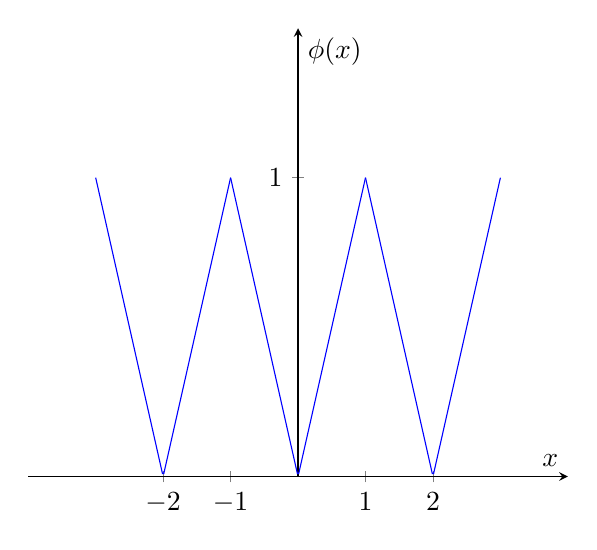
\begin{tikzpicture}
			\begin{axis}[
					axis lines=middle,
					xlabel={$x$},
					ylabel={$\phi(x)$},
					xtick={-2, -1, 0, 1, 2},
					xticklabels={$-2$, $-1$, $0$, $1$, $2$},
					ytick={0, 1},
					yticklabels={$0$, $1$},
					ymin=0,
					ymax=1.5,
					xmin=-4,
					xmax=4,
				]
				\addplot[domain=-1:1, samples=100, color=blue]{abs(x)};
				\addplot[domain=1:3, samples=100, color=blue]{abs(x-2)};
				\addplot[domain=-3:-1, samples=100, color=blue]{abs(x+2)};
			\end{axis}
		\end{tikzpicture}
	\end{center}
	Then $\phi$ is continuous on $\R$, and in fact, $\left|\phi(x)-\phi(y)\right|\le \left|x-y\right|$ for all $x,y \in \R$ (Lipschitz bound).\\
	Let
	\begin{flalign*}
		f_n(x) & =\sum_{k=0}^{n}{{\left(\frac{3}{4}\right)}^{n}\phi(4^{n}x)}                                \\
		f(x)   & = \lim_{n\to \infty}{f_n(x)}=\sum_{n=0}^{\infty}{\left(\frac{3}{4}\right)^{n}\phi(4^{n}x)}
		.\end{flalign*}
	Then the series $f(x)$ converges uniformly on $\R$ by the Weierstrass M-test (Theorem~\ref{thm:7.10}) since $\left|\left(\frac{3}{4}\right)^{n}\phi(4^{n}x)\right|\le \left(\frac{3}{4}\right)^{n}$ and $\sum_{n=0}^{\infty}{\left(\frac{3}{4}\right)^{n}}<\infty$.\\

	Also, $f$ is continuous on $\R$ by Corollary~\ref{cor:7.12}.\\
	Claim: $f'(x)$ does not exist for any $x \in \R$.\\
	It suffices to show that for $x \in \R$, there exists $\delta_m\to 0$  s.t. \[
		\left|\underbrace{\frac{f(x+\delta_m)-f(x)}{\delta_m}}_{= \sum_{n=0}^{\infty}{{\frac{3}{4}}^{n}\gamma_n}, \gamma_n= \frac{\phi(4^{n}(x+\delta_m))-\phi(4^{n}x)}{\delta_m}}\right| \to  \infty \text{ as } m\to \infty
		.\]
	Note
	\[
		4^m \left( x + \delta_m \right) = 4^m x - \frac{1}{2}
		,\]
	\[
		4^m \left( x + 1 - \delta_m \right) = 4^m x + \frac{1}{2}
		.\]
	Choose $\delta_m=\pm \frac{1}{2} \cdot 4^{-m}$ with sign chosen (depending on $x$) so that there is no integer between $4^m x$ and $4^m (x+\delta_m)$.\\
	\begin{center}
		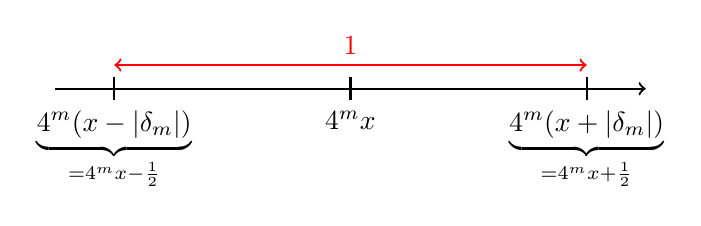
\begin{tikzpicture}[thick, scale=1.5]
			% Draw the number line
			\draw[->] (-2.5, 0) -- (2.5, 0);

			% Draw the intervals and points
			\draw[-] (0, -0.1) -- (0, 0.1);
			\node[below] at (0, -0.1) {\(4^m x\)};

			\draw[-] (-2, -0.1) -- (-2, 0.1);
			\node[below] at (-2, -0.1) {\(\underbrace{4^m (x - \left|\delta_m\right|)}_{=4^{m}x-\frac{1}{2}}\)};

			\draw[-] (2, -0.1) -- (2, 0.1);
			\node[below] at (2, -0.1) {\(\underbrace{4^m (x + \left|\delta_m\right|)}_{=4^{m}x+\frac{1}{2}}\)};

			\node[above, red] at (0, 0.2) {\(1\)};

			\draw[<-, red] (-2, 0.2) -- (0, 0.2);
			\draw[->, red] (0, 0.2) -- (2, 0.2);
		\end{tikzpicture}
	\end{center}
	Then $\gamma_n=0$ if $n\neq m$ and $\gamma_m=\frac{\phi(4^{m}(x+4^{-m}))- \phi(4^{m}x)}{4^{-m}}$.
	In particular, \[
		\left|\phi(4^{m}(x+\delta_m))-\phi(4^{m}x)\right| =\left|4^{m} \delta_m\right| =\frac{1}{2}
		.\]
	If $n>m$, then \[
		\phi(4^{n}(x+\delta_m))-\phi(4^{m}x)=\phi(4^{n}x \pm \underbrace{4^{n}\cdot \frac{1}{2}\cdot \frac{1}{4^{m}}}_{\text{even integer}})-\phi(4^{m}x)=0
		.\]
	Hence, $\gamma_n=0$ for $n>m$.\\
	Since $\phi(x)-\phi(y)\le \left|x-y\right| $, for $n\le m$,
	\[
		\gamma_n\le  \frac{1}{\left|\delta_m\right|} \cdot \left|4^{m}\delta_m\right| =4^{m}
		.\]
	In fact, $\left|\gamma_m\right| =\frac{1}{\left|\delta_m\right| }\cdot \frac{1}{2}=4^{m}$.\\
	Therefore,
	\begin{flalign*}
		\left|\frac{f(x+\delta_m)-f(x)}{\delta_m}\right| & = \left|\sum_{n=0}^{\infty}{\left(\frac{3}{4}\right)^{n}\gamma_n} \right|
		=\left|\sum_{n=0}^{m}{\left(\frac{3}{4}\right)^{n} \gamma_n}\right|                                                                                                             \\
		                                                 & \ge \left(\frac{3}{4}\right)^{m} \left|\gamma_m\right| -\sum_{n=0}^{m-1}{\left(\frac{3}{4}\right)^{n} \left|\gamma_n\right|} \\ & \ge \left(\frac{3}{4}\right)^{m} \cdot 4^{m}-\sum_{n=0}^{m-1}{\left(\frac{3}{4}\right)^{n}4^{n}} \\
		                                                 & =3^{m}-\frac{3^{m}-1}{3-1}=\frac{1}{2}(3^{m}+1)\to \infty \text{ as } m\to \infty
		.\end{flalign*}
\end{proof}
\begin{define}[Equicontinuity]
	A family $\mathscr{F}$ of functions on $E$ is equicontinuous if $\forall{\epsilon > 0}: \exists{\delta > 0} \text{ s.t. } f \in  \mathscr{F}; x,y \in E; d(x,y)<\delta\implies  \left|f(x)-f(y)\right| < \epsilon$.
	\begin{remark}
		\begin{enumerate}
			\item If $\mathscr{F}$ is equicontinuous, then every ${f \in  \mathscr{F}}$ is uniformly continuous on $E$.
			\item Any finite set of uniformly continuous functions is equicontinuous.
		\end{enumerate}
	\end{remark}
	\begin{example}
		Let $\mathscr{F}=\{f_1,f_2,\ldots \}$, where $f_n(x)=\frac{\sin{nx}}{\sqrt{n}}$, $x \in E=[0,1]$. We have seen $f_n\to 0$ uniformly on $E$.\\
		Claim $\mathscr{F}$ is equicontinuous.\\
		Let $\epsilon>0$. Choose $N$ s.t. $\frac{2}{\sqrt{n}}<\epsilon$ for all $n\ge N$.\\
		Since $\{f_1,f_2,\ldots f_{N-1}\}$ is a finite set of uniformly continuous functions, it is equicontinuous.\\
		Hence, $\exists{\delta>0} \text{ s.t. } n<N \text{ and } \left|x-y\right| <\delta\implies \left|f_n(x)-f_n(y)\right| <\epsilon$.\\
		Therefore, $n \in \N$ and $\left|x-y\right| < \delta \implies \left|f_n(x)-f_n(y)<\right| \epsilon$.
	\end{example}
\end{define}

\begin{problem}[7.16]
Let $\{f_n\}$ be an equicontinuous sequence of functions $f_n:K\to \C$, where $K$ is compact.\\
Suppose $\lim_{n\to \infty}{f_n(x)}=f(x)$ exists for all $x \in K$. Then $f_n\to f$ uniformly on $K$.
\begin{proof}
	We use $\frac{\epsilon}{3}$ argument.\\
	Let $\epsilon>0$. $\exists{\delta > 0} \text{ s.t. } \left|f_n(x)-f_n(y)\right| <\frac{\epsilon}{3}$ for all $x,y \in K$ s.t. $d(x,y)<\delta$ and $n \in \N$.\\
	Since $K$ is compact, the open cover $\{N_{\delta}(x)\}_{x \in K}$ has a finite subcover $\{N_{\delta}(x_1),\ldots,N_{\delta}(x_k)\}$.\\
	Thus, given any $x \in K$, $\exists j \text{ s.t. } d(x,x_j)<\delta$. Then,
	\begin{flalign*}
		\left|f_n(x)-f_m(x)\right| & \le \underbrace{\left|f_n(x)-f_n(x_j)\right|}_{<\frac{\epsilon}{3}} +\left|f_n(x_j)-f_m(x_j)\right| +\underbrace{\left|f_m(x_j)-f_m(x)\right|}_{<\frac{\epsilon}{3}}
		.\end{flalign*}
	For each $i=1,\ldots ,k$, we know $\{f_n(x_i)\}_n$ is a convergent sequence, so it's a Cauchy sequence. Hence, $\exists{N_i} \text{ s.t. } m,n\ge N_i\implies \left|f_m(x_i)-f_n(x_i)\right|<\frac{\epsilon}{3}$.\\
	Let $N=\max\{N_1,N_2,\ldots ,N_k\} $. Then \[
		m,n\ge N\implies \left|f_m(x)-f_n(x)\right| <\frac{\epsilon}{3}+\frac{\epsilon}{3}+\frac{\epsilon}{3} =\epsilon
		.\]
	Therefore, $f_{n}\to f$ uniformly on $K$.
\end{proof}
\end{problem}


\begin{thm}[24]
	If $f_{n}: K\to \C$ are continuous and $K$ is compact and $f_{n}\to f$ uniformly on $K$, then $\{f_{n}\}$ is equicontinuous.
	\begin{proof}
		(Using $\frac{\epsilon}{3}$ argument)\\
		Let $\epsilon>0$. Since $f_{n}\to f$ uniformly, $\exists{N} \text{ s.t. } $ $m,n\ge N \implies \left|f_{m}(x)-f_{n}(x)\right|<\frac{\epsilon}{3}$  for all $x \in K$. Since $K$ is compact, each $f_{n}$ is uniformly continuous.
		Hence, $\{f_1,\ldots ,f_{N}\} $ is equicontinuous, so $\exists{\delta >0} \text{ s.t. } \left|f_{i}(x)-f_{i}(y)\right| <\frac{\epsilon}{3}$ if $d(x,y)<\delta$ for all $i \in \{1,2,\ldots ,N\}$.\\
		For $n\ge N$,
		\[
			\left| f_{n}(x)-f_{n}(y)\right| \le \underbrace{\left|f_{n}(x)-f_{N}(x)\right|} _{<\frac{\epsilon}{3}}+ \underbrace{\left|f_N(x)-f_N(y)\right|}_{<\frac{\epsilon}{3} \text{ if } d(x,y)<\delta}+\underbrace{\left|f_N(y)-f_n(y)\right|}_{<\frac{\epsilon}{3}}<\epsilon \text{ if } d(x,y)<\delta
			.\]
	\end{proof}
\end{thm}

\begin{example}
	Let \[
		f_{n}(x)=\begin{cases}
			2nx    & 0\le x< \frac{1}{2n}           \\
			-2nx+2 & \frac{1}{2n}\le x< \frac{1}{n} \\
			0      & \frac{1}{n}\le x\le 1
		\end{cases}
		.\]
	\begin{center}
		\begin{tikzpicture}
			\begin{axis}[
					axis lines=middle,
					xlabel={$x$},
					ylabel={$y=f_n(x)$},
					xtick={0, 0.5, 1},
					xticklabels={$0$, $\frac{1}{2n}$, $\frac{1}{n}$},
					ytick={0, 1},
					yticklabels={$0$, $1$},
					ymin=0,
					ymax=1.5,
					xmin=-0.1,
					xmax=2,
				]
				\addplot[domain=0:0.5, samples=100, color=blue]{2*x};
				\addplot[domain=0.5:1, samples=100, color=blue]{-2*x+2};
				\addplot[domain=1:1.8, samples=100, color=blue]{0};
			\end{axis}
		\end{tikzpicture}
	\end{center}
	$\{f_{n}\}$ obeys $\left|f_{n}(x)\right| \le 1$ for all $ n \in \N, x \in [0,1]$. It is not equicontinuous because $\left|f_{n}(\frac{1}{2n})-f_{n}(0)\right|=1-0=1$ for all $n$. Also, no subsequence of $\{f_{n}\} $ can converge uniformly since $f_{n}(\frac{1}{2n})=1$ whereas $\lim_{n\to \infty}{f_{n}(x)}=0$ for all $x \in [0,1]$.
\end{example}

\begin{define}[7.19]
	\label{def:7.19}
	\begin{enumerate}
		\item $\{f_{n}\}$ is pointwise bounded on $E$ if $\exists{\phi : E\to \R} \text{ s.t. } \left|f_{n}(x)\right|{<} \phi(x) $ for all $n \in \N, x \in E$.\\
		      Note: $<$ can be replaced with $\le $ but Rudin uses strict inequality
		\item $\{f_{n}\}$ is uniformly bounded on $E$ if $\exists{M>0} \text{ s.t. } \left|f_{n}(x)\right|<M$ for all $n \in \N, x \in E$.
	\end{enumerate}
\end{define}

\begin{example}
	Let \[
		f_{n}(x)=\frac{1}{x}+\frac{1}{n}, n \in \N, x \in E=(0,1].
		.\]
	Then $f_n(x)$ is pointwise bounded on $E$ since $\left|f_{n}(x)\right|<\frac{1}{x}+2$ for all $n \in \N, x \in E$.\\
	However, $\{f_{n}\}$ is not uniformly bounded on $E$ since $f_{n}(x)>\frac{1}{x}$ and $\frac{1}{x}\to \infty$ as $x\to 0^{+}$.
\end{example}

\begin{thm}[23][Selection Theorem]
	Suppose $E$ is a countable set and $f_{n}:E\to \C$ is pointwise bounded.
	Then there exists $\{f_{n_k}\}$ of $\{ {f}_{n}\} $ which is pointwise convergent on $E$; i.e., \[
		\lim_{k\to \infty}{\{ {f}_{n_{k}}(x)\}} \text{ exists for all } x \in E
		.\]
	\begin{proof}
		(Using diagonal argument)\\
		Let $E=\{x_1,x_2,x_3,\ldots \}$.\\
		Since $\{{f}_{n}(x_1)\}_{n}$ is bounded, $\exists{\text{ subsequence }\{f_{1,k}\}} \text{ s.t. } \lim_{k\to \infty}{f_{1,k}(x_1)}$ exists by Weierstrass theorem~\ref{thm:2.42}.\\
		Successive subsequences can be constructed as follows:\\
		\begin{flalign*}
			S_1 & : f_{1,1},f_{1,2},f_{1,3},f_{1,4},\ldots \text{ converges on $x_1$}          \\
			S_2 & : f_{2,1},f_{2,2},f_{2,3},f_{2,4},\ldots \text{ converges on $x_1, x_2$}     \\
			S_3 & : f_{3,1},f_{3,2},f_{3,3},f_{3,4},\ldots \text{ converges on $x_1, x_2,x_3$} \\
			    & \vdots                                                                       \\.
		\end{flalign*}
		Note we can make $S_n$ converges not just on $x_n$ but also for $\{x_1,x_2,\ldots ,x_{n-1}\}$ by taking a subsequence of $S_{n-1}$.\\
		This is because $f_{n-1, k}$ is also a pointwise bounded sequence itself.\\
		Form a diagonal subsequence $S: f_{1,1}, f_{2,2}, f_{3,3}, f_{4,4}, \ldots $.
		Then $S$ is eventually a subsequence of each $S_j$, so it converges on $x_1,x_2,x_3,\ldots ,x_j$. This is true for all $j$, so $\{f_{n,n}(x_i)\}_n $ converges for each $x_{i} \in E$.
	\end{proof}
\end{thm}

\begin{lemma}
	If $K$ is compact then $K$ has a countable dense subset $E \subset K$; i.e., $\overline{E} = K$, or $\forall{p \in K}: \forall{r > 0}: \exists{x \in E} \text{ s.t. } d(p,x)<r$.
	We also say $K$ is separable. See Problem 2.25.
	\begin{proof}
		For $n \in \N$, $\{N_{\frac{1}{n}}(p)\}_{p \in K}$ is an open cover of $K$, so $\exists $ finite subcover $\{N_{\frac{1}{n}}(p)\}_{p \in E_{n}}$, $E_{n} \subset K$, $E_{n}$ finite. Let $E= \bigcup_{n=1}^{\infty} E_n$, a countable set.\\
		Let $p \in K$ and $r >0$. Choose $n_0$ s.t. $\frac{1}{n_0}<r$.\\
		By definition of $E_{n_0}$, there exists $x_0 \in E_{n_0}$ s.t. $p \in N_{\frac{1}{n_0}}(x_0)$.\\
		Then $d(p,x_0)<\frac{1}{n_0}<r$, so $E$ is dense in $K$.
	\end{proof}
\end{lemma}


\begin{thm}[25]
	Suppose $K$ is compact and that $\mathscr{F}=\{f_{n}\} \subset \mathscr{C}(K)$ is equicontinuous and pointwise bounded on $K$. Then
	\begin{enumerate}
		\item $\{f_{n}\} $ is uniformly bounded
		\item $\{f_{n}\}$ has a uniformly convergent subsequence; i.e., a subsequence that converges uniformly in $(\mathscr{C}(K), \|\cdot\|)$
	\end{enumerate}
	\begin{remark}
		\begin{enumerate}[label=\arabic*.]
			\item  A more topological statement: A5.3
			\item Converse: [(b)$\implies$ equicontinuity and uniform boundedness] see A5.4
			\item need for compactness of $K$: see A5.5
			\item good theorem/proof to master..
		\end{enumerate}
	\end{remark}
	\begin{proof}
		\begin{enumerate}
			\item Goal: Find $M$ s.t. $\left|f_{n}(x)\right| \le M	 \text{ for all } n \in \N, x \in K$.\\
			      Since $\mathscr{F}$ is equicontinuous,
			      \[
				      \forall{\epsilon > 0}: \exists{\delta > 0} \text{ s.t. } \forall{n \in \N}: d(x,y)<\delta \implies \left|f_{n}(x)-f_{n}(y)\right|<\epsilon
				      .\]
			      As $K$ is compact, $\exists{\{p_1,p_2,\ldots ,p_{n}\} \in K} \text{ s.t. } \{N_{\delta}(p_{i})\}_{i \in \{1,\ldots,r\}}$ covers $K$. Given $x \in K$, choose $p_{i}$ s.t. $x \in N_{\delta}(p_{i})$.\\
			      For each $i$, $\{f_{n}(p_{i})\}_n$ is bounded, say $\left|f_{n}(p_{i})\right|\le M_i$ for all $n \in \N$.\\
			      Let $M_0=\max\{M_1,\ldots ,M_r\}$. Then $\left|f_{n}(x)\right|\le \left|f_{n}(p_{i})\right|+\left|f_{n}(x)-f_{n}(p_{i})\right| \le M_0+\epsilon=M$ (can take $\epsilon=1$ in part (a)).
			\item Goal: Construct a uniformly convergent subsequence of $\{ {f}_{n}\}$.\\
			      Step 1. By the lemma, $K$ has a countable dense subset $E \subset K$.\\
			      By Theorem~\ref{thm:7.23}, $\exists{\{f_{n_i}\}}$ s.t. $\lim_{i\to \infty}{f_{n_i}(x)}$ exists for all $x \in E$.
			      Write $g_{i}=f_{n_i}$. We show $g_i$ converges uniformly on $K$ via the Uniform Cauchy Criterion Theorem~\ref{thm:7.8}.\\
			      Step 2. Let $\epsilon>0$. By equicontinuity, $\exists{\delta > 0} \text{ s.t. } d(x,y) < \delta \implies \left|g_{i}(x)-g_{i}(y)\right|<\frac{\epsilon}{3}$ for all $i$.\\
			      $\{ {N}_{\delta}(p)\}_{p \in E}$ covers $K$ since $E$ is dense.
			      There exists a finite subcover $\{N_{\delta}(x_1),\ldots ,N_{\delta}(x_{m})\}$ with each $x_s \in E$. Given $x \in K$ there exists $x_s$ s.t. $d(x,x_s)<\delta$.\\
			      Step 3. (using $\frac{\epsilon}{3}$ argument)\\
			      \begin{flalign*}
				      g_{i}(x)-g_{j}(x) & \le \underbrace{\left|g_{i}(x)-g_{i}(x_s)\right|}_{<\frac{\epsilon}{3} \;\; (\because d(x,x_s)<\delta)} + \left|g_{i}(x_s)-g_{j}(x_s)\right| + \underbrace{\left|g_{j}(x_s)-g_{j}(x)\right|}_{<\frac{\epsilon}{3}}
				      .\end{flalign*}

			      Since $\lim_{i\to \infty}{\{g_{i}(x)\}}$ converges for any $x \in K$, $\{g_{i}(x_s)\}_i$ is a Cauchy sequence.\\
			      % Since $\{g_{i}(x_{s})\}_i$ converges
			      Hence for $s=1,\ldots ,m$, we can choose $N_s$ s.t. $ i,j\ge N_{s}\implies \left|g_{i}(x_{s})-g_{j}(x_{s})\right| <\frac{\epsilon}{3}$.\\
			      Let $N= \max\{N_1,\ldots ,N_m\}$. Then for $i,j\ge N (\text{independent of }x)$,
			      \[
				      \left|g_i(x)-g_j(x)\right|<\frac{\epsilon}{3}+\frac{\epsilon}{3}+\frac{\epsilon}{3}
				      .\]
			      Hence, $\{g_{i}\}$ converges uniformly on $K$ by Theorem~\ref{thm:7.8}.
		\end{enumerate}
	\end{proof}
\end{thm}


\begin{thm}[26][Weierstrass's Theorem]
	Let $f: [a,b]\to \R (\text{ or } \C)$ be continuous.\\
	There exists polynomials $p_{n}$ s.t. $p_{n}\to f$ uniformly on $[a,b]$.

\end{thm}

